\documentclass[1p]{elsarticle_modified}
%\bibliographystyle{elsarticle-num}

%\usepackage[colorlinks]{hyperref}
%\usepackage{abbrmath_seonhwa} %\Abb, \Ascr, \Acal ,\Abf, \Afrak
\usepackage{amsfonts}
\usepackage{amssymb}
\usepackage{amsmath}
\usepackage{amsthm}
\usepackage{scalefnt}
\usepackage{amsbsy}
\usepackage{kotex}
\usepackage{caption}
\usepackage{subfig}
\usepackage{color}
\usepackage{graphicx}
\usepackage{xcolor} %% white, black, red, green, blue, cyan, magenta, yellow
\usepackage{float}
\usepackage{setspace}
\usepackage{hyperref}

\usepackage{tikz}
\usetikzlibrary{arrows}

\usepackage{multirow}
\usepackage{array} % fixed length table
\usepackage{hhline}

%%%%%%%%%%%%%%%%%%%%%
\makeatletter
\renewcommand*\env@matrix[1][\arraystretch]{%
	\edef\arraystretch{#1}%
	\hskip -\arraycolsep
	\let\@ifnextchar\new@ifnextchar
	\array{*\c@MaxMatrixCols c}}
\makeatother %https://tex.stackexchange.com/questions/14071/how-can-i-increase-the-line-spacing-in-a-matrix
%%%%%%%%%%%%%%%

\usepackage[normalem]{ulem}

\newcommand{\msout}[1]{\ifmmode\text{\sout{\ensuremath{#1}}}\else\sout{#1}\fi}
%SOURCE: \msout is \stkout macro in https://tex.stackexchange.com/questions/20609/strikeout-in-math-mode

\newcommand{\cancel}[1]{
	\ifmmode
	{\color{red}\msout{#1}}
	\else
	{\color{red}\sout{#1}}
	\fi
}

\newcommand{\add}[1]{
	{\color{blue}\uwave{#1}}
}

\newcommand{\replace}[2]{
	\ifmmode
	{\color{red}\msout{#1}}{\color{blue}\uwave{#2}}
	\else
	{\color{red}\sout{#1}}{\color{blue}\uwave{#2}}
	\fi
}

\newcommand{\Sol}{\mathcal{S}} %segment
\newcommand{\D}{D} %diagram
\newcommand{\A}{\mathcal{A}} %arc


%%%%%%%%%%%%%%%%%%%%%%%%%%%%%5 test

\def\sl{\operatorname{\textup{SL}}(2,\Cbb)}
\def\psl{\operatorname{\textup{PSL}}(2,\Cbb)}
\def\quan{\mkern 1mu \triangleright \mkern 1mu}

\theoremstyle{definition}
\newtheorem{thm}{Theorem}[section]
\newtheorem{prop}[thm]{Proposition}
\newtheorem{lem}[thm]{Lemma}
\newtheorem{ques}[thm]{Question}
\newtheorem{cor}[thm]{Corollary}
\newtheorem{defn}[thm]{Definition}
\newtheorem{exam}[thm]{Example}
\newtheorem{rmk}[thm]{Remark}
\newtheorem{alg}[thm]{Algorithm}

\newcommand{\I}{\sqrt{-1}}
\begin{document}

%\begin{frontmatter}
%
%\title{Boundary parabolic representations of knots up to 8 crossings}
%
%%% Group authors per affiliation:
%\author{Yunhi Cho} 
%\address{Department of Mathematics, University of Seoul, Seoul, Korea}
%\ead{yhcho@uos.ac.kr}
%
%
%\author{Seonhwa Kim} %\fnref{s_kim}}
%\address{Center for Geometry and Physics, Institute for Basic Science, Pohang, 37673, Korea}
%\ead{ryeona17@ibs.re.kr}
%
%\author{Hyuk Kim}
%\address{Department of Mathematical Sciences, Seoul National University, Seoul 08826, Korea}
%\ead{hyukkim@snu.ac.kr}
%
%\author{Seokbeom Yoon}
%\address{Department of Mathematical Sciences, Seoul National University, Seoul, 08826,  Korea}
%\ead{sbyoon15@snu.ac.kr}
%
%\begin{abstract}
%We find all boundary parabolic representation of knots up to 8 crossings.
%
%\end{abstract}
%\begin{keyword}
%    \MSC[2010] 57M25 
%\end{keyword}
%
%\end{frontmatter}

%\linenumbers
%\tableofcontents
%
\newcommand\colored[1]{\textcolor{white}{\rule[-0.35ex]{0.8em}{1.4ex}}\kern-0.8em\color{red} #1}%
%\newcommand\colored[1]{\textcolor{white}{ #1}\kern-2.17ex	\textcolor{white}{ #1}\kern-1.81ex	\textcolor{white}{ #1}\kern-2.15ex\color{red}#1	}

{\Large $\underline{12n_{0438}~(K12n_{0438})}$}

\setlength{\tabcolsep}{10pt}
\renewcommand{\arraystretch}{1.6}
\vspace{1cm}\begin{tabular}{m{100pt}>{\centering\arraybackslash}m{274pt}}
\multirow{5}{120pt}{
	\centering
	\includegraphics[width=112pt]{../../../GIT/diagram.site/Diagrams/png/2527_12n_0438.png}\\
\ \ \ A knot diagram\footnotemark}&
\allowdisplaybreaks
\textbf{Linearized knot diagam} \\
\cline{2-2}
 &
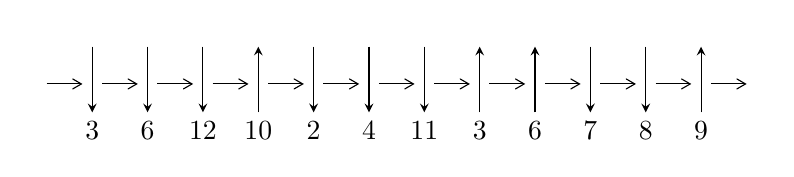
\begin{tikzpicture}[x=20pt, y=17pt]
	% nodes
	\node (C0) at (0, 0) {};
	\node (C1) at (1, 0) {};
	\node (C1U) at (1, +1) {};
	\node (C1D) at (1, -1) {3};

	\node (C2) at (2, 0) {};
	\node (C2U) at (2, +1) {};
	\node (C2D) at (2, -1) {6};

	\node (C3) at (3, 0) {};
	\node (C3U) at (3, +1) {};
	\node (C3D) at (3, -1) {12};

	\node (C4) at (4, 0) {};
	\node (C4U) at (4, +1) {};
	\node (C4D) at (4, -1) {10};

	\node (C5) at (5, 0) {};
	\node (C5U) at (5, +1) {};
	\node (C5D) at (5, -1) {2};

	\node (C6) at (6, 0) {};
	\node (C6U) at (6, +1) {};
	\node (C6D) at (6, -1) {4};

	\node (C7) at (7, 0) {};
	\node (C7U) at (7, +1) {};
	\node (C7D) at (7, -1) {11};

	\node (C8) at (8, 0) {};
	\node (C8U) at (8, +1) {};
	\node (C8D) at (8, -1) {3};

	\node (C9) at (9, 0) {};
	\node (C9U) at (9, +1) {};
	\node (C9D) at (9, -1) {6};

	\node (C10) at (10, 0) {};
	\node (C10U) at (10, +1) {};
	\node (C10D) at (10, -1) {7};

	\node (C11) at (11, 0) {};
	\node (C11U) at (11, +1) {};
	\node (C11D) at (11, -1) {8};

	\node (C12) at (12, 0) {};
	\node (C12U) at (12, +1) {};
	\node (C12D) at (12, -1) {9};
	\node (C13) at (13, 0) {};

	% arrows
	\draw[->,>={angle 60}]
	(C0) edge (C1) (C1) edge (C2) (C2) edge (C3) (C3) edge (C4) (C4) edge (C5) (C5) edge (C6) (C6) edge (C7) (C7) edge (C8) (C8) edge (C9) (C9) edge (C10) (C10) edge (C11) (C11) edge (C12) (C12) edge (C13) ;	\draw[->,>=stealth]
	(C1U) edge (C1D) (C2U) edge (C2D) (C3U) edge (C3D) (C4D) edge (C4U) (C5U) edge (C5D) (C6U) edge (C6D) (C7U) edge (C7D) (C8D) edge (C8U) (C9D) edge (C9U) (C10U) edge (C10D) (C11U) edge (C11D) (C12D) edge (C12U) ;
	\end{tikzpicture} \\
\hhline{~~} \\& 
\textbf{Solving Sequence} \\ \cline{2-2} 
 &
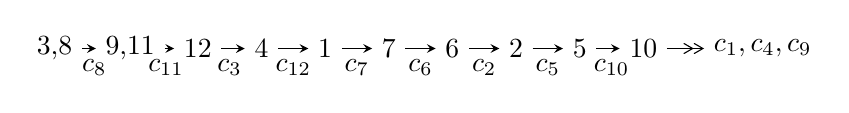
\begin{tikzpicture}[x=23pt, y=7pt]
	% node
	\node (A0) at (-1/8, 0) {3,8};
	\node (A1) at (17/16, 0) {9,11};
	\node (A2) at (17/8, 0) {12};
	\node (A3) at (25/8, 0) {4};
	\node (A4) at (33/8, 0) {1};
	\node (A5) at (41/8, 0) {7};
	\node (A6) at (49/8, 0) {6};
	\node (A7) at (57/8, 0) {2};
	\node (A8) at (65/8, 0) {5};
	\node (A9) at (73/8, 0) {10};
	\node (C1) at (1/2, -1) {$c_{8}$};
	\node (C2) at (13/8, -1) {$c_{11}$};
	\node (C3) at (21/8, -1) {$c_{3}$};
	\node (C4) at (29/8, -1) {$c_{12}$};
	\node (C5) at (37/8, -1) {$c_{7}$};
	\node (C6) at (45/8, -1) {$c_{6}$};
	\node (C7) at (53/8, -1) {$c_{2}$};
	\node (C8) at (61/8, -1) {$c_{5}$};
	\node (C9) at (69/8, -1) {$c_{10}$};
	\node (A10) at (11, 0) {$c_{1},c_{4},c_{9}$};

	% edge
	\draw[->,>=stealth]	
	(A0) edge (A1) (A1) edge (A2) (A2) edge (A3) (A3) edge (A4) (A4) edge (A5) (A5) edge (A6) (A6) edge (A7) (A7) edge (A8) (A8) edge (A9) ;
	\draw[->>,>={angle 60}]	
	(A9) edge (A10);
\end{tikzpicture} \\ 

\end{tabular} \\

\footnotetext{
The image of knot diagram is generated by the software ``\textbf{Draw programme}" developed by Andrew Bartholomew(\url{http://www.layer8.co.uk/maths/draw/index.htm\#Running-draw}), where we modified some parts for our purpose(\url{https://github.com/CATsTAILs/LinksPainter}).
}\phantom \\ \newline 
\centering \textbf{Ideals for irreducible components\footnotemark of $X_{\text{par}}$} 
 
\begin{align*}
I^u_{1}&=\langle 
9586 u^{11}-3055 u^{10}+\cdots+9038 b-18587,\;-55772 u^{11}+21076 u^{10}+\cdots+4519 a+136449,\\
\phantom{I^u_{1}}&\phantom{= \langle  }u^{12}+9 u^{10}+u^9+13 u^8+3 u^7-37 u^6-8 u^5- u^4+13 u^3+7 u^2-2 u-1\rangle \\
I^u_{2}&=\langle 
23 u^7-19 u^6+114 u^5-105 u^4+47 u^3-42 u^2+83 b-10 u-77,\\
\phantom{I^u_{2}}&\phantom{= \langle  }67 u^7-77 u^6+379 u^5-443 u^4+422 u^3-310 u^2+83 a+191 u-347,\;u^8+6 u^6+8 u^4+3 u^3+7 u^2+u+1\rangle \\
I^u_{3}&=\langle 
220741 u^{11}+352170 u^{10}+\cdots+4894159 b+8758441,\\
\phantom{I^u_{3}}&\phantom{= \langle  }-6799412 u^{11}+191458 u^{10}+\cdots+4894159 a+38864844,\\
\phantom{I^u_{3}}&\phantom{= \langle  }u^{12}+13 u^{10}- u^9+61 u^8-7 u^7+121 u^6-12 u^5+96 u^4-21 u^3+34 u^2-5 u+1\rangle \\
I^u_{4}&=\langle 
- u^2+b+u-1,\;- u^3+u^2+a-2 u+2,\;u^4-2 u^3+3 u^2-2 u-1\rangle \\
I^u_{5}&=\langle 
b,\;a+u,\;u^2+u+1\rangle \\
\\
\end{align*}
\raggedright * 5 irreducible components of $\dim_{\mathbb{C}}=0$, with total 38 representations.\\
\footnotetext{All coefficients of polynomials are rational numbers. But the coefficients are sometimes approximated in decimal forms when there is not enough margin.}
\newpage
\renewcommand{\arraystretch}{1}
\centering \section*{I. $I^u_{1}= \langle 9586 u^{11}-3055 u^{10}+\cdots+9038 b-18587,\;-55772 u^{11}+21076 u^{10}+\cdots+4519 a+136449,\;u^{12}+9 u^{10}+\cdots-2 u-1 \rangle$}
\flushleft \textbf{(i) Arc colorings}\\
\begin{tabular}{m{7pt} m{180pt} m{7pt} m{180pt} }
\flushright $a_{3}=$&$\begin{pmatrix}0\\u\end{pmatrix}$ \\
\flushright $a_{8}=$&$\begin{pmatrix}1\\0\end{pmatrix}$ \\
\flushright $a_{9}=$&$\begin{pmatrix}1\\- u^2\end{pmatrix}$ \\
\flushright $a_{11}=$&$\begin{pmatrix}12.3417 u^{11}-4.66386 u^{10}+\cdots+18.7431 u-30.1945\\-1.06063 u^{11}+0.338017 u^{10}+\cdots-1.12669 u+2.05654\end{pmatrix}$ \\
\flushright $a_{12}=$&$\begin{pmatrix}13.4023 u^{11}-5.00188 u^{10}+\cdots+19.8698 u-32.2511\\-1.06063 u^{11}+0.338017 u^{10}+\cdots-1.12669 u+2.05654\end{pmatrix}$ \\
\flushright $a_{4}=$&$\begin{pmatrix}-7.52003 u^{11}+3.05964 u^{10}+\cdots-7.40042 u+16.9010\\-3.22129 u^{11}+1.14240 u^{10}+\cdots-3.67039 u+7.94722\end{pmatrix}$ \\
\flushright $a_{1}=$&$\begin{pmatrix}14.4826 u^{11}-5.40407 u^{10}+\cdots+22.1416 u-35.1964\\-1.23069 u^{11}+0.347201 u^{10}+\cdots-1.40263 u+2.45873\end{pmatrix}$ \\
\flushright $a_{7}=$&$\begin{pmatrix}6.68843 u^{11}-2.59150 u^{10}+\cdots+10.4001 u-16.2423\\-1.25880 u^{11}+0.629785 u^{10}+\cdots-1.01427 u+3.32253\end{pmatrix}$ \\
\flushright $a_{6}=$&$\begin{pmatrix}-7.16254 u^{11}+2.94534 u^{10}+\cdots-8.99015 u+20.2930\\- u\end{pmatrix}$ \\
\flushright $a_{2}=$&$\begin{pmatrix}14.4826 u^{11}-5.40407 u^{10}+\cdots+22.1416 u-35.1964\\1.08033 u^{11}-0.402191 u^{10}+\cdots+2.27185 u-2.94534\end{pmatrix}$ \\
\flushright $a_{5}=$&$\begin{pmatrix}10.9114 u^{11}-4.21122 u^{10}+\cdots+11.3468 u-25.2504\\3.39135 u^{11}-1.15158 u^{10}+\cdots+3.94634 u-8.34941\end{pmatrix}$ \\
\flushright $a_{10}=$&$\begin{pmatrix}8.34941 u^{11}-3.39135 u^{10}+\cdots+12.1990 u-20.6452\\0.402191 u^{11}-0.170060 u^{10}+\cdots+0.784687 u-1.08033\end{pmatrix}$\\&\end{tabular}
\flushleft \textbf{(ii) Obstruction class $= -1$}\\~\\
\flushleft \textbf{(iii) Cusp Shapes $= \frac{37615}{9038} u^{11}-\frac{13351}{4519} u^{10}+\frac{172836}{4519} u^9-\frac{209101}{9038} u^8+\frac{263227}{4519} u^7-\frac{290229}{9038} u^6-\frac{1386017}{9038} u^5+\frac{583207}{9038} u^4-\frac{56976}{4519} u^3+\frac{639833}{9038} u^2-\frac{58931}{9038} u-\frac{151555}{9038}$}\\~\\
\newpage\renewcommand{\arraystretch}{1}
\flushleft \textbf{(iv) u-Polynomials at the component}\newline \\
\begin{tabular}{m{50pt}|m{274pt}}
Crossings & \hspace{64pt}u-Polynomials at each crossing \\
\hline $$\begin{aligned}c_{1}\end{aligned}$$&$\begin{aligned}
&u^{12}+37 u^{11}+\cdots+6273 u+64
\end{aligned}$\\
\hline $$\begin{aligned}c_{2},c_{5}\end{aligned}$$&$\begin{aligned}
&u^{12}+9 u^{11}+\cdots-57 u+8
\end{aligned}$\\
\hline $$\begin{aligned}c_{3},c_{6}\end{aligned}$$&$\begin{aligned}
&u^{12}-2 u^{11}+\cdots-3 u-1
\end{aligned}$\\
\hline $$\begin{aligned}c_{4},c_{8}\end{aligned}$$&$\begin{aligned}
&u^{12}+9 u^{10}- u^9+13 u^8-3 u^7-37 u^6+8 u^5- u^4-13 u^3+7 u^2+2 u-1
\end{aligned}$\\
\hline $$\begin{aligned}c_{7},c_{10},c_{11}\end{aligned}$$&$\begin{aligned}
&u^{12}+6 u^{11}+\cdots+7 u-2
\end{aligned}$\\
\hline $$\begin{aligned}c_{9},c_{12}\end{aligned}$$&$\begin{aligned}
&u^{12}+u^{11}+\cdots+36 u+1
\end{aligned}$\\
\hline
\end{tabular}\\~\\
\newpage\renewcommand{\arraystretch}{1}
\flushleft \textbf{(v) Riley Polynomials at the component}\newline \\
\begin{tabular}{m{50pt}|m{274pt}}
Crossings & \hspace{64pt}Riley Polynomials at each crossing \\
\hline $$\begin{aligned}c_{1}\end{aligned}$$&$\begin{aligned}
&y^{12}-233 y^{11}+\cdots-38719361 y+4096
\end{aligned}$\\
\hline $$\begin{aligned}c_{2},c_{5}\end{aligned}$$&$\begin{aligned}
&y^{12}-37 y^{11}+\cdots-6273 y+64
\end{aligned}$\\
\hline $$\begin{aligned}c_{3},c_{6}\end{aligned}$$&$\begin{aligned}
&y^{12}-6 y^{11}+\cdots+y+1
\end{aligned}$\\
\hline $$\begin{aligned}c_{4},c_{8}\end{aligned}$$&$\begin{aligned}
&y^{12}+18 y^{11}+\cdots-18 y+1
\end{aligned}$\\
\hline $$\begin{aligned}c_{7},c_{10},c_{11}\end{aligned}$$&$\begin{aligned}
&y^{12}-12 y^{11}+\cdots-109 y+4
\end{aligned}$\\
\hline $$\begin{aligned}c_{9},c_{12}\end{aligned}$$&$\begin{aligned}
&y^{12}+45 y^{11}+\cdots-670 y+1
\end{aligned}$\\
\hline
\end{tabular}\\~\\
\newpage\flushleft \textbf{(vi) Complex Volumes and Cusp Shapes}
$$\begin{array}{c|c|c}  
\text{Solutions to }I^u_{1}& \I (\text{vol} + \sqrt{-1}CS) & \text{Cusp shape}\\
 \hline 
\begin{aligned}
u &= \phantom{-}1.04860\phantom{ +0.000000I} \\
a &= \phantom{-}3.26000\phantom{ +0.000000I} \\
b &= \phantom{-}1.86936\phantom{ +0.000000I}\end{aligned}
 & -8.03214\phantom{ +0.000000I} & -11.1250\phantom{ +0.000000I} \\ \hline\begin{aligned}
u &= -1.19673\phantom{ +0.000000I} \\
a &= \phantom{-}0.457184\phantom{ +0.000000I} \\
b &= \phantom{-}1.40652\phantom{ +0.000000I}\end{aligned}
 & -6.56513\phantom{ +0.000000I} & -13.9820\phantom{ +0.000000I} \\ \hline\begin{aligned}
u &= \phantom{-}0.785212\phantom{ +0.000000I} \\
a &= \phantom{-}0.538255\phantom{ +0.000000I} \\
b &= \phantom{-}1.39001\phantom{ +0.000000I}\end{aligned}
 & -3.33445\phantom{ +0.000000I} & -1.37130\phantom{ +0.000000I} \\ \hline\begin{aligned}
u &= -0.237929 + 0.713496 I \\
a &= \phantom{-}0.839776 + 0.248914 I \\
b &= \phantom{-}0.549193 + 0.617015 I\end{aligned}
 & -0.28261 - 1.48442 I & -3.85780 + 2.07743 I \\ \hline\begin{aligned}
u &= -0.237929 - 0.713496 I \\
a &= \phantom{-}0.839776 - 0.248914 I \\
b &= \phantom{-}0.549193 - 0.617015 I\end{aligned}
 & -0.28261 + 1.48442 I & -3.85780 - 2.07743 I \\ \hline\begin{aligned}
u &= \phantom{-}0.413934\phantom{ +0.000000I} \\
a &= \phantom{-}1.40772\phantom{ +0.000000I} \\
b &= -0.208689\phantom{ +0.000000I}\end{aligned}
 & -1.36886\phantom{ +0.000000I} & -8.24790\phantom{ +0.000000I} \\ \hline\begin{aligned}
u &= -0.398984 + 0.012900 I \\
a &= -1.37647 - 2.67835 I \\
b &= -0.666632 + 0.239214 I\end{aligned}
 & \phantom{-}1.97549 - 2.44144 I & \phantom{-}0.80466 - 1.29895 I \\ \hline\begin{aligned}
u &= -0.398984 - 0.012900 I \\
a &= -1.37647 + 2.67835 I \\
b &= -0.666632 - 0.239214 I\end{aligned}
 & \phantom{-}1.97549 + 2.44144 I & \phantom{-}0.80466 + 1.29895 I \\ \hline\begin{aligned}
u &= -0.05938 + 2.26410 I \\
a &= -1.045270 - 0.699289 I \\
b &= -0.85675 - 1.28813 I\end{aligned}
 & -15.6479 - 4.2966 I & -9.24517 + 3.48018 I \\ \hline\begin{aligned}
u &= -0.05938 - 2.26410 I \\
a &= -1.045270 + 0.699289 I \\
b &= -0.85675 + 1.28813 I\end{aligned}
 & -15.6479 + 4.2966 I & -9.24517 - 3.48018 I\\
 \hline 
 \end{array}$$\newpage$$\begin{array}{c|c|c}  
\text{Solutions to }I^u_{1}& \I (\text{vol} + \sqrt{-1}CS) & \text{Cusp shape}\\
 \hline 
\begin{aligned}
u &= \phantom{-}0.17079 + 2.29628 I \\
a &= \phantom{-}2.25039 + 0.29367 I \\
b &= \phantom{-}1.74558 - 0.39261 I\end{aligned}
 & \phantom{-}15.3806 + 10.5658 I & -8.83901 - 3.88482 I \\ \hline\begin{aligned}
u &= \phantom{-}0.17079 - 2.29628 I \\
a &= \phantom{-}2.25039 - 0.29367 I \\
b &= \phantom{-}1.74558 + 0.39261 I\end{aligned}
 & \phantom{-}15.3806 - 10.5658 I & -8.83901 + 3.88482 I\\
 \hline 
 \end{array}$$\newpage\newpage\renewcommand{\arraystretch}{1}
\centering \section*{II. $I^u_{2}= \langle 23 u^7-19 u^6+\cdots+83 b-77,\;67 u^7-77 u^6+\cdots+83 a-347,\;u^8+6 u^6+8 u^4+3 u^3+7 u^2+u+1 \rangle$}
\flushleft \textbf{(i) Arc colorings}\\
\begin{tabular}{m{7pt} m{180pt} m{7pt} m{180pt} }
\flushright $a_{3}=$&$\begin{pmatrix}0\\u\end{pmatrix}$ \\
\flushright $a_{8}=$&$\begin{pmatrix}1\\0\end{pmatrix}$ \\
\flushright $a_{9}=$&$\begin{pmatrix}1\\- u^2\end{pmatrix}$ \\
\flushright $a_{11}=$&$\begin{pmatrix}-0.807229 u^{7}+0.927711 u^{6}+\cdots-2.30120 u+4.18072\\-0.277108 u^{7}+0.228916 u^{6}+\cdots+0.120482 u+0.927711\end{pmatrix}$ \\
\flushright $a_{12}=$&$\begin{pmatrix}-0.530120 u^{7}+0.698795 u^{6}+\cdots-2.42169 u+3.25301\\-0.277108 u^{7}+0.228916 u^{6}+\cdots+0.120482 u+0.927711\end{pmatrix}$ \\
\flushright $a_{4}=$&$\begin{pmatrix}-1.74699 u^{7}-0.469880 u^{6}+\cdots-10.4578 u-3.32530\\-0.301205 u^{7}-0.0120482 u^{6}+\cdots-2.21687 u-0.469880\end{pmatrix}$ \\
\flushright $a_{1}=$&$\begin{pmatrix}-0.819277 u^{7}+0.807229 u^{6}+\cdots-2.46988 u+3.48193\\-0.361446 u^{7}+0.385542 u^{6}+\cdots-0.0602410 u+1.03614\end{pmatrix}$ \\
\flushright $a_{7}=$&$\begin{pmatrix}0.542169 u^{7}-0.578313 u^{6}+\cdots+1.59036 u-2.55422\\0.0722892 u^{7}-0.277108 u^{6}+\cdots+0.0120482 u-0.807229\end{pmatrix}$ \\
\flushright $a_{6}=$&$\begin{pmatrix}-1.27711 u^{7}+0.228916 u^{6}+\cdots-6.87952 u+0.927711\\- u\end{pmatrix}$ \\
\flushright $a_{2}=$&$\begin{pmatrix}-0.819277 u^{7}+0.807229 u^{6}+\cdots-2.46988 u+3.48193\\-0.289157 u^{7}+0.108434 u^{6}+\cdots-0.0481928 u+0.228916\end{pmatrix}$ \\
\flushright $a_{5}=$&$\begin{pmatrix}-1.96386 u^{7}-0.638554 u^{6}+\cdots-12.4940 u-3.90361\\-0.216867 u^{7}-0.168675 u^{6}+\cdots-2.03614 u-0.578313\end{pmatrix}$ \\
\flushright $a_{10}=$&$\begin{pmatrix}-0.578313 u^{7}+0.216867 u^{6}+\cdots-2.09639 u+1.45783\\-0.108434 u^{7}-0.0843373 u^{6}+\cdots-0.518072 u-0.289157\end{pmatrix}$\\&\end{tabular}
\flushleft \textbf{(ii) Obstruction class $= 1$}\\~\\
\flushleft \textbf{(iii) Cusp Shapes $= \frac{277}{83} u^7+\frac{114}{83} u^6+\frac{1640}{83} u^5+\frac{547}{83} u^4+\frac{2042}{83} u^3+\frac{999}{83} u^2+\frac{2052}{83} u-\frac{285}{83}$}\\~\\
\newpage\renewcommand{\arraystretch}{1}
\flushleft \textbf{(iv) u-Polynomials at the component}\newline \\
\begin{tabular}{m{50pt}|m{274pt}}
Crossings & \hspace{64pt}u-Polynomials at each crossing \\
\hline $$\begin{aligned}c_{1}\end{aligned}$$&$\begin{aligned}
&u^8-8 u^7+18 u^6-9 u^5+31 u^4+18 u^3+14 u^2+3 u+1
\end{aligned}$\\
\hline $$\begin{aligned}c_{2}\end{aligned}$$&$\begin{aligned}
&u^8+6 u^7+14 u^6+17 u^5+13 u^4+8 u^3+6 u^2+3 u+1
\end{aligned}$\\
\hline $$\begin{aligned}c_{3},c_{6}\end{aligned}$$&$\begin{aligned}
&u^8+2 u^7+2 u^6-2 u^4-3 u^3+2 u+1
\end{aligned}$\\
\hline $$\begin{aligned}c_{4},c_{8}\end{aligned}$$&$\begin{aligned}
&u^8+6 u^6+8 u^4+3 u^3+7 u^2+u+1
\end{aligned}$\\
\hline $$\begin{aligned}c_{5}\end{aligned}$$&$\begin{aligned}
&u^8-6 u^7+14 u^6-17 u^5+13 u^4-8 u^3+6 u^2-3 u+1
\end{aligned}$\\
\hline $$\begin{aligned}c_{7}\end{aligned}$$&$\begin{aligned}
&u^8+3 u^7+u^6-3 u^5+u^3-4 u^2- u+3
\end{aligned}$\\
\hline $$\begin{aligned}c_{9},c_{12}\end{aligned}$$&$\begin{aligned}
&u^8- u^7+8 u^6- u^5+14 u^4+5 u^3+7 u^2+5 u+1
\end{aligned}$\\
\hline $$\begin{aligned}c_{10},c_{11}\end{aligned}$$&$\begin{aligned}
&u^8-3 u^7+u^6+3 u^5- u^3-4 u^2+u+3
\end{aligned}$\\
\hline
\end{tabular}\\~\\
\newpage\renewcommand{\arraystretch}{1}
\flushleft \textbf{(v) Riley Polynomials at the component}\newline \\
\begin{tabular}{m{50pt}|m{274pt}}
Crossings & \hspace{64pt}Riley Polynomials at each crossing \\
\hline $$\begin{aligned}c_{1}\end{aligned}$$&$\begin{aligned}
&y^8-28 y^7+242 y^6+1351 y^5+1839 y^4+634 y^3+150 y^2+19 y+1
\end{aligned}$\\
\hline $$\begin{aligned}c_{2},c_{5}\end{aligned}$$&$\begin{aligned}
&y^8-8 y^7+18 y^6-9 y^5+31 y^4+18 y^3+14 y^2+3 y+1
\end{aligned}$\\
\hline $$\begin{aligned}c_{3},c_{6}\end{aligned}$$&$\begin{aligned}
&y^8+4 y^5-2 y^4-5 y^3+8 y^2-4 y+1
\end{aligned}$\\
\hline $$\begin{aligned}c_{4},c_{8}\end{aligned}$$&$\begin{aligned}
&y^8+12 y^7+52 y^6+110 y^5+150 y^4+115 y^3+59 y^2+13 y+1
\end{aligned}$\\
\hline $$\begin{aligned}c_{7},c_{10},c_{11}\end{aligned}$$&$\begin{aligned}
&y^8-7 y^7+19 y^6-23 y^5+10 y^4- y^3+18 y^2-25 y+9
\end{aligned}$\\
\hline $$\begin{aligned}c_{9},c_{12}\end{aligned}$$&$\begin{aligned}
&y^8+15 y^7+90 y^6+247 y^5+330 y^4+197 y^3+27 y^2-11 y+1
\end{aligned}$\\
\hline
\end{tabular}\\~\\
\newpage\flushleft \textbf{(vi) Complex Volumes and Cusp Shapes}
$$\begin{array}{c|c|c}  
\text{Solutions to }I^u_{2}& \I (\text{vol} + \sqrt{-1}CS) & \text{Cusp shape}\\
 \hline 
\begin{aligned}
u &= -0.452128 + 0.754240 I \\
a &= \phantom{-}0.281547 + 0.149763 I \\
b &= \phantom{-}0.364928 + 0.928632 I\end{aligned}
 & -0.91626 - 2.11958 I & -9.09548 + 6.29610 I \\ \hline\begin{aligned}
u &= -0.452128 - 0.754240 I \\
a &= \phantom{-}0.281547 - 0.149763 I \\
b &= \phantom{-}0.364928 - 0.928632 I\end{aligned}
 & -0.91626 + 2.11958 I & -9.09548 - 6.29610 I \\ \hline\begin{aligned}
u &= \phantom{-}0.588231 + 1.086850 I \\
a &= -1.70900 - 0.76306 I \\
b &= -1.56785 + 0.26923 I\end{aligned}
 & -7.73259 + 6.48719 I & -6.82312 - 5.90005 I \\ \hline\begin{aligned}
u &= \phantom{-}0.588231 - 1.086850 I \\
a &= -1.70900 + 0.76306 I \\
b &= -1.56785 - 0.26923 I\end{aligned}
 & -7.73259 - 6.48719 I & -6.82312 + 5.90005 I \\ \hline\begin{aligned}
u &= -0.051535 + 0.424185 I \\
a &= \phantom{-}3.68516 - 0.74169 I \\
b &= \phantom{-}0.862997 + 0.073353 I\end{aligned}
 & \phantom{-}1.63676 - 2.95067 I & -6.12574 + 8.48868 I \\ \hline\begin{aligned}
u &= -0.051535 - 0.424185 I \\
a &= \phantom{-}3.68516 + 0.74169 I \\
b &= \phantom{-}0.862997 - 0.073353 I\end{aligned}
 & \phantom{-}1.63676 + 2.95067 I & -6.12574 - 8.48868 I \\ \hline\begin{aligned}
u &= -0.08457 + 2.15179 I \\
a &= -1.257710 - 0.086043 I \\
b &= -1.160080 - 0.491572 I\end{aligned}
 & -14.3720 - 2.0722 I & -9.45567 + 2.68473 I \\ \hline\begin{aligned}
u &= -0.08457 - 2.15179 I \\
a &= -1.257710 + 0.086043 I \\
b &= -1.160080 + 0.491572 I\end{aligned}
 & -14.3720 + 2.0722 I & -9.45567 - 2.68473 I\\
 \hline 
 \end{array}$$\newpage\newpage\renewcommand{\arraystretch}{1}
\centering \section*{III. $I^u_{3}= \langle 2.21\times10^{5} u^{11}+3.52\times10^{5} u^{10}+\cdots+4.89\times10^{6} b+8.76\times10^{6},\;-6.80\times10^{6} u^{11}+1.91\times10^{5} u^{10}+\cdots+4.89\times10^{6} a+3.89\times10^{7},\;u^{12}+13 u^{10}+\cdots-5 u+1 \rangle$}
\flushleft \textbf{(i) Arc colorings}\\
\begin{tabular}{m{7pt} m{180pt} m{7pt} m{180pt} }
\flushright $a_{3}=$&$\begin{pmatrix}0\\u\end{pmatrix}$ \\
\flushright $a_{8}=$&$\begin{pmatrix}1\\0\end{pmatrix}$ \\
\flushright $a_{9}=$&$\begin{pmatrix}1\\- u^2\end{pmatrix}$ \\
\flushright $a_{11}=$&$\begin{pmatrix}1.38929 u^{11}-0.0391197 u^{10}+\cdots+43.9779 u-7.94107\\-0.0451029 u^{11}-0.0719572 u^{10}+\cdots-0.177550 u-1.78957\end{pmatrix}$ \\
\flushright $a_{12}=$&$\begin{pmatrix}1.43439 u^{11}+0.0328375 u^{10}+\cdots+44.1554 u-6.15150\\-0.0451029 u^{11}-0.0719572 u^{10}+\cdots-0.177550 u-1.78957\end{pmatrix}$ \\
\flushright $a_{4}=$&$\begin{pmatrix}1.86149 u^{11}+0.0277566 u^{10}+\cdots+56.7778 u-7.54448\\-0.0255782 u^{11}-0.108973 u^{10}+\cdots+1.02646 u-2.23971\end{pmatrix}$ \\
\flushright $a_{1}=$&$\begin{pmatrix}1.35518 u^{11}-0.0779405 u^{10}+\cdots+42.7077 u-7.97390\\-0.0413761 u^{11}-0.131233 u^{10}+\cdots+0.297122 u-1.90035\end{pmatrix}$ \\
\flushright $a_{7}=$&$\begin{pmatrix}2.16779 u^{11}-0.0984377 u^{10}+\cdots+66.0594 u-12.7530\\-0.0719229 u^{11}-0.0728595 u^{10}+\cdots-2.91466 u-2.58092\end{pmatrix}$ \\
\flushright $a_{6}=$&$\begin{pmatrix}0.740548 u^{11}+0.241490 u^{10}+\cdots+20.0889 u+4.36298\\0.434394 u^{11}+0.0328375 u^{10}+\cdots+11.1554 u-1.15150\end{pmatrix}$ \\
\flushright $a_{2}=$&$\begin{pmatrix}1.35518 u^{11}-0.0779405 u^{10}+\cdots+42.7077 u-7.97390\\-0.0792181 u^{11}-0.110778 u^{10}+\cdots-1.44776 u-1.82241\end{pmatrix}$ \\
\flushright $a_{5}=$&$\begin{pmatrix}2.02148 u^{11}+0.591926 u^{10}+\cdots+56.7443 u+8.63238\\0.902855 u^{11}+0.0689238 u^{10}+\cdots+24.8073 u-2.82600\end{pmatrix}$ \\
\flushright $a_{10}=$&$\begin{pmatrix}-1.74447 u^{11}+0.117060 u^{10}+\cdots-53.6856 u+13.9150\\0.286593 u^{11}+0.0646620 u^{10}+\cdots+8.24327 u+2.04902\end{pmatrix}$\\&\end{tabular}
\flushleft \textbf{(ii) Obstruction class $= -1$}\\~\\
\flushleft \textbf{(iii) Cusp Shapes $= \frac{1038229}{4894159} u^{11}-\frac{453029}{4894159} u^{10}+\cdots+\frac{62859079}{4894159} u-\frac{46129032}{4894159}$}\\~\\
\newpage\renewcommand{\arraystretch}{1}
\flushleft \textbf{(iv) u-Polynomials at the component}\newline \\
\begin{tabular}{m{50pt}|m{274pt}}
Crossings & \hspace{64pt}u-Polynomials at each crossing \\
\hline $$\begin{aligned}c_{1}\end{aligned}$$&$\begin{aligned}
&(u^6+8 u^5-53 u^3+58 u^2-15 u+9)^2
\end{aligned}$\\
\hline $$\begin{aligned}c_{2},c_{5}\end{aligned}$$&$\begin{aligned}
&(u^6-4 u^5+4 u^4-3 u^3+4 u^2+3 u+3)^2
\end{aligned}$\\
\hline $$\begin{aligned}c_{3},c_{6}\end{aligned}$$&$\begin{aligned}
&u^{12}-4 u^{11}+\cdots+u+1
\end{aligned}$\\
\hline $$\begin{aligned}c_{4},c_{8}\end{aligned}$$&$\begin{aligned}
&u^{12}+13 u^{10}+\cdots+5 u+1
\end{aligned}$\\
\hline $$\begin{aligned}c_{7},c_{10},c_{11}\end{aligned}$$&$\begin{aligned}
&(u^6- u^5-4 u^4+3 u^3+4 u^2-2)^2
\end{aligned}$\\
\hline $$\begin{aligned}c_{9},c_{12}\end{aligned}$$&$\begin{aligned}
&u^{12}-3 u^{11}+\cdots-8 u+173
\end{aligned}$\\
\hline
\end{tabular}\\~\\
\newpage\renewcommand{\arraystretch}{1}
\flushleft \textbf{(v) Riley Polynomials at the component}\newline \\
\begin{tabular}{m{50pt}|m{274pt}}
Crossings & \hspace{64pt}Riley Polynomials at each crossing \\
\hline $$\begin{aligned}c_{1}\end{aligned}$$&$\begin{aligned}
&(y^6-64 y^5+964 y^4-2551 y^3+1774 y^2+819 y+81)^2
\end{aligned}$\\
\hline $$\begin{aligned}c_{2},c_{5}\end{aligned}$$&$\begin{aligned}
&(y^6-8 y^5+53 y^3+58 y^2+15 y+9)^2
\end{aligned}$\\
\hline $$\begin{aligned}c_{3},c_{6}\end{aligned}$$&$\begin{aligned}
&y^{12}-2 y^{11}+\cdots+23 y+1
\end{aligned}$\\
\hline $$\begin{aligned}c_{4},c_{8}\end{aligned}$$&$\begin{aligned}
&y^{12}+26 y^{11}+\cdots+43 y+1
\end{aligned}$\\
\hline $$\begin{aligned}c_{7},c_{10},c_{11}\end{aligned}$$&$\begin{aligned}
&(y^6-9 y^5+30 y^4-45 y^3+32 y^2-16 y+4)^2
\end{aligned}$\\
\hline $$\begin{aligned}c_{9},c_{12}\end{aligned}$$&$\begin{aligned}
&y^{12}+29 y^{11}+\cdots+170514 y+29929
\end{aligned}$\\
\hline
\end{tabular}\\~\\
\newpage\flushleft \textbf{(vi) Complex Volumes and Cusp Shapes}
$$\begin{array}{c|c|c}  
\text{Solutions to }I^u_{3}& \I (\text{vol} + \sqrt{-1}CS) & \text{Cusp shape}\\
 \hline 
\begin{aligned}
u &= -0.374731 + 0.890342 I \\
a &= \phantom{-}1.185720 - 0.141464 I \\
b &= \phantom{-}0.629305 + 0.469465 I\end{aligned}
 & -0.31318 - 1.57342 I & -5.93222 + 3.43140 I \\ \hline\begin{aligned}
u &= -0.374731 - 0.890342 I \\
a &= \phantom{-}1.185720 + 0.141464 I \\
b &= \phantom{-}0.629305 - 0.469465 I\end{aligned}
 & -0.31318 + 1.57342 I & -5.93222 - 3.43140 I \\ \hline\begin{aligned}
u &= \phantom{-}0.219901 + 0.674731 I \\
a &= \phantom{-}0.347492 + 0.244157 I \\
b &= \phantom{-}0.629305 + 0.469465 I\end{aligned}
 & -0.31318 - 1.57342 I & -5.93222 + 3.43140 I \\ \hline\begin{aligned}
u &= \phantom{-}0.219901 - 0.674731 I \\
a &= \phantom{-}0.347492 - 0.244157 I \\
b &= \phantom{-}0.629305 - 0.469465 I\end{aligned}
 & -0.31318 + 1.57342 I & -5.93222 - 3.43140 I \\ \hline\begin{aligned}
u &= \phantom{-}0.32643 + 1.59597 I \\
a &= -2.15982 - 0.63392 I \\
b &= -1.63022 + 0.19616 I\end{aligned}
 & -8.12771 + 4.22943 I & -8.28340 - 1.79030 I \\ \hline\begin{aligned}
u &= \phantom{-}0.32643 - 1.59597 I \\
a &= -2.15982 + 0.63392 I \\
b &= -1.63022 - 0.19616 I\end{aligned}
 & -8.12771 - 4.22943 I & -8.28340 + 1.79030 I \\ \hline\begin{aligned}
u &= \phantom{-}0.080159 + 0.164473 I \\
a &= -4.43127 + 6.14837 I \\
b &= -1.63022 - 0.19616 I\end{aligned}
 & -8.12771 - 4.22943 I & -8.28340 + 1.79030 I \\ \hline\begin{aligned}
u &= \phantom{-}0.080159 - 0.164473 I \\
a &= -4.43127 - 6.14837 I \\
b &= -1.63022 + 0.19616 I\end{aligned}
 & -8.12771 + 4.22943 I & -8.28340 - 1.79030 I \\ \hline\begin{aligned}
u &= -0.37385 + 2.16844 I \\
a &= \phantom{-}2.53178 + 0.44785 I \\
b &= \phantom{-}1.70687\phantom{ +0.000000I}\end{aligned}
 & \phantom{-}16.3722\phantom{ +0.000000I} & -8.87611 + 0. I\phantom{ +0.000000I} \\ \hline\begin{aligned}
u &= -0.37385 - 2.16844 I \\
a &= \phantom{-}2.53178 - 0.44785 I \\
b &= \phantom{-}1.70687\phantom{ +0.000000I}\end{aligned}
 & \phantom{-}16.3722\phantom{ +0.000000I} & -8.87611 + 0. I\phantom{ +0.000000I}\\
 \hline 
 \end{array}$$\newpage$$\begin{array}{c|c|c}  
\text{Solutions to }I^u_{3}& \I (\text{vol} + \sqrt{-1}CS) & \text{Cusp shape}\\
 \hline 
\begin{aligned}
u &= \phantom{-}0.12209 + 2.22085 I \\
a &= -0.973901 + 0.448921 I \\
b &= -0.705047\phantom{ +0.000000I}\end{aligned}
 & -14.2948\phantom{ +0.000000I} & -8.69265 + 0. I\phantom{ +0.000000I} \\ \hline\begin{aligned}
u &= \phantom{-}0.12209 - 2.22085 I \\
a &= -0.973901 - 0.448921 I \\
b &= -0.705047\phantom{ +0.000000I}\end{aligned}
 & -14.2948\phantom{ +0.000000I} & -8.69265 + 0. I\phantom{ +0.000000I}\\
 \hline 
 \end{array}$$\newpage\newpage\renewcommand{\arraystretch}{1}
\centering \section*{IV. $I^u_{4}= \langle - u^2+b+u-1,\;- u^3+u^2+a-2 u+2,\;u^4-2 u^3+3 u^2-2 u-1 \rangle$}
\flushleft \textbf{(i) Arc colorings}\\
\begin{tabular}{m{7pt} m{180pt} m{7pt} m{180pt} }
\flushright $a_{3}=$&$\begin{pmatrix}0\\u\end{pmatrix}$ \\
\flushright $a_{8}=$&$\begin{pmatrix}1\\0\end{pmatrix}$ \\
\flushright $a_{9}=$&$\begin{pmatrix}1\\- u^2\end{pmatrix}$ \\
\flushright $a_{11}=$&$\begin{pmatrix}u^3- u^2+2 u-2\\u^2- u+1\end{pmatrix}$ \\
\flushright $a_{12}=$&$\begin{pmatrix}u^3-2 u^2+3 u-3\\u^2- u+1\end{pmatrix}$ \\
\flushright $a_{4}=$&$\begin{pmatrix}- u^3+2 u^2-4 u+4\\u^3-2 u^2+3 u-1\end{pmatrix}$ \\
\flushright $a_{1}=$&$\begin{pmatrix}u^3-2 u^2+3 u-2\\- u+1\end{pmatrix}$ \\
\flushright $a_{7}=$&$\begin{pmatrix}- u^3+3 u^2-5 u+3\\-2\end{pmatrix}$ \\
\flushright $a_{6}=$&$\begin{pmatrix}- u^3+2 u^2-3 u+2\\u-1\end{pmatrix}$ \\
\flushright $a_{2}=$&$\begin{pmatrix}u^3-2 u^2+3 u-2\\1\end{pmatrix}$ \\
\flushright $a_{5}=$&$\begin{pmatrix}0\\u\end{pmatrix}$ \\
\flushright $a_{10}=$&$\begin{pmatrix}- u^3+2 u^2-3 u+3\\- u^2+u-1\end{pmatrix}$\\&\end{tabular}
\flushleft \textbf{(ii) Obstruction class $= 1$}\\~\\
\flushleft \textbf{(iii) Cusp Shapes $= -8$}\\~\\
\newpage\renewcommand{\arraystretch}{1}
\flushleft \textbf{(iv) u-Polynomials at the component}\newline \\
\begin{tabular}{m{50pt}|m{274pt}}
Crossings & \hspace{64pt}u-Polynomials at each crossing \\
\hline $$\begin{aligned}c_{1},c_{2}\end{aligned}$$&$\begin{aligned}
&(u-1)^4
\end{aligned}$\\
\hline $$\begin{aligned}c_{3},c_{6}\end{aligned}$$&$\begin{aligned}
&u^4+2 u^3+3 u^2+2 u-1
\end{aligned}$\\
\hline $$\begin{aligned}c_{4},c_{8}\end{aligned}$$&$\begin{aligned}
&u^4-2 u^3+3 u^2-2 u-1
\end{aligned}$\\
\hline $$\begin{aligned}c_{5},c_{9},c_{12}\end{aligned}$$&$\begin{aligned}
&(u+1)^4
\end{aligned}$\\
\hline $$\begin{aligned}c_{7},c_{10},c_{11}\end{aligned}$$&$\begin{aligned}
&(u^2-2)^2
\end{aligned}$\\
\hline
\end{tabular}\\~\\
\newpage\renewcommand{\arraystretch}{1}
\flushleft \textbf{(v) Riley Polynomials at the component}\newline \\
\begin{tabular}{m{50pt}|m{274pt}}
Crossings & \hspace{64pt}Riley Polynomials at each crossing \\
\hline $$\begin{aligned}c_{1},c_{2},c_{5}\\c_{9},c_{12}\end{aligned}$$&$\begin{aligned}
&(y-1)^4
\end{aligned}$\\
\hline $$\begin{aligned}c_{3},c_{4},c_{6}\\c_{8}\end{aligned}$$&$\begin{aligned}
&y^4+2 y^3- y^2-10 y+1
\end{aligned}$\\
\hline $$\begin{aligned}c_{7},c_{10},c_{11}\end{aligned}$$&$\begin{aligned}
&(y-2)^4
\end{aligned}$\\
\hline
\end{tabular}\\~\\
\newpage\flushleft \textbf{(vi) Complex Volumes and Cusp Shapes}
$$\begin{array}{c|c|c}  
\text{Solutions to }I^u_{4}& \I (\text{vol} + \sqrt{-1}CS) & \text{Cusp shape}\\
 \hline 
\begin{aligned}
u &= \phantom{-}1.31499\phantom{ +0.000000I} \\
a &= \phantom{-}1.17467\phantom{ +0.000000I} \\
b &= \phantom{-}1.41421\phantom{ +0.000000I}\end{aligned}
 & -4.93480\phantom{ +0.000000I} & -8.00000\phantom{ +0.000000I} \\ \hline\begin{aligned}
u &= \phantom{-}0.50000 + 1.47113 I \\
a &= -2.20711 - 0.60936 I \\
b &= -1.41421\phantom{ +0.000000I}\end{aligned}
 & -4.93480\phantom{ +0.000000I} & -8.00000\phantom{ +0.000000I} \\ \hline\begin{aligned}
u &= \phantom{-}0.50000 - 1.47113 I \\
a &= -2.20711 + 0.60936 I \\
b &= -1.41421\phantom{ +0.000000I}\end{aligned}
 & -4.93480\phantom{ +0.000000I} & -8.00000\phantom{ +0.000000I} \\ \hline\begin{aligned}
u &= -0.314993\phantom{ +0.000000I} \\
a &= -2.76046\phantom{ +0.000000I} \\
b &= \phantom{-}1.41421\phantom{ +0.000000I}\end{aligned}
 & -4.93480\phantom{ +0.000000I} & -8.00000\phantom{ +0.000000I}\\
 \hline 
 \end{array}$$\newpage\newpage\renewcommand{\arraystretch}{1}
\centering \section*{V. $I^u_{5}= \langle b,\;a+u,\;u^2+u+1 \rangle$}
\flushleft \textbf{(i) Arc colorings}\\
\begin{tabular}{m{7pt} m{180pt} m{7pt} m{180pt} }
\flushright $a_{3}=$&$\begin{pmatrix}0\\u\end{pmatrix}$ \\
\flushright $a_{8}=$&$\begin{pmatrix}1\\0\end{pmatrix}$ \\
\flushright $a_{9}=$&$\begin{pmatrix}1\\u+1\end{pmatrix}$ \\
\flushright $a_{11}=$&$\begin{pmatrix}- u\\0\end{pmatrix}$ \\
\flushright $a_{12}=$&$\begin{pmatrix}- u\\0\end{pmatrix}$ \\
\flushright $a_{4}=$&$\begin{pmatrix}-1\\u\end{pmatrix}$ \\
\flushright $a_{1}=$&$\begin{pmatrix}- u-1\\- u-1\end{pmatrix}$ \\
\flushright $a_{7}=$&$\begin{pmatrix}1\\0\end{pmatrix}$ \\
\flushright $a_{6}=$&$\begin{pmatrix}u+1\\u+1\end{pmatrix}$ \\
\flushright $a_{2}=$&$\begin{pmatrix}- u-1\\-1\end{pmatrix}$ \\
\flushright $a_{5}=$&$\begin{pmatrix}0\\u\end{pmatrix}$ \\
\flushright $a_{10}=$&$\begin{pmatrix}- u\\0\end{pmatrix}$\\&\end{tabular}
\flushleft \textbf{(ii) Obstruction class $= 1$}\\~\\
\flushleft \textbf{(iii) Cusp Shapes $= -6$}\\~\\
\newpage\renewcommand{\arraystretch}{1}
\flushleft \textbf{(iv) u-Polynomials at the component}\newline \\
\begin{tabular}{m{50pt}|m{274pt}}
Crossings & \hspace{64pt}u-Polynomials at each crossing \\
\hline $$\begin{aligned}c_{1},c_{2},c_{9}\\c_{12}\end{aligned}$$&$\begin{aligned}
&(u-1)^2
\end{aligned}$\\
\hline $$\begin{aligned}c_{3},c_{4},c_{6}\\c_{8}\end{aligned}$$&$\begin{aligned}
&u^2+u+1
\end{aligned}$\\
\hline $$\begin{aligned}c_{5}\end{aligned}$$&$\begin{aligned}
&(u+1)^2
\end{aligned}$\\
\hline $$\begin{aligned}c_{7},c_{10},c_{11}\end{aligned}$$&$\begin{aligned}
&u^2
\end{aligned}$\\
\hline
\end{tabular}\\~\\
\newpage\renewcommand{\arraystretch}{1}
\flushleft \textbf{(v) Riley Polynomials at the component}\newline \\
\begin{tabular}{m{50pt}|m{274pt}}
Crossings & \hspace{64pt}Riley Polynomials at each crossing \\
\hline $$\begin{aligned}c_{1},c_{2},c_{5}\\c_{9},c_{12}\end{aligned}$$&$\begin{aligned}
&(y-1)^2
\end{aligned}$\\
\hline $$\begin{aligned}c_{3},c_{4},c_{6}\\c_{8}\end{aligned}$$&$\begin{aligned}
&y^2+y+1
\end{aligned}$\\
\hline $$\begin{aligned}c_{7},c_{10},c_{11}\end{aligned}$$&$\begin{aligned}
&y^2
\end{aligned}$\\
\hline
\end{tabular}\\~\\
\newpage\flushleft \textbf{(vi) Complex Volumes and Cusp Shapes}
$$\begin{array}{c|c|c}  
\text{Solutions to }I^u_{5}& \I (\text{vol} + \sqrt{-1}CS) & \text{Cusp shape}\\
 \hline 
\begin{aligned}
u &= -0.500000 + 0.866025 I \\
a &= \phantom{-}0.500000 - 0.866025 I \\
b &= \phantom{-0.000000 } 0\end{aligned}
 & \phantom{-0.000000 } 0 & -6.00000\phantom{ +0.000000I} \\ \hline\begin{aligned}
u &= -0.500000 - 0.866025 I \\
a &= \phantom{-}0.500000 + 0.866025 I \\
b &= \phantom{-0.000000 } 0\end{aligned}
 & \phantom{-0.000000 } 0 & -6.00000\phantom{ +0.000000I}\\
 \hline 
 \end{array}$$\newpage
\newpage\renewcommand{\arraystretch}{1}
\centering \section*{ VI. u-Polynomials}
\begin{tabular}{m{50pt}|m{274pt}}
Crossings & \hspace{64pt}u-Polynomials at each crossing \\
\hline $$\begin{aligned}c_{1}\end{aligned}$$&$\begin{aligned}
&(u-1)^6(u^6+8 u^5-53 u^3+58 u^2-15 u+9)^2\\
&\cdot(u^8-8 u^7+18 u^6-9 u^5+31 u^4+18 u^3+14 u^2+3 u+1)\\
&\cdot(u^{12}+37 u^{11}+\cdots+6273 u+64)
\end{aligned}$\\
\hline $$\begin{aligned}c_{2}\end{aligned}$$&$\begin{aligned}
&(u-1)^6(u^6-4 u^5+4 u^4-3 u^3+4 u^2+3 u+3)^2\\
&\cdot(u^8+6 u^7+14 u^6+17 u^5+13 u^4+8 u^3+6 u^2+3 u+1)\\
&\cdot(u^{12}+9 u^{11}+\cdots-57 u+8)
\end{aligned}$\\
\hline $$\begin{aligned}c_{3},c_{6}\end{aligned}$$&$\begin{aligned}
&(u^2+u+1)(u^4+2 u^3+\cdots+2 u-1)(u^8+2 u^7+\cdots+2 u+1)\\
&\cdot(u^{12}-4 u^{11}+\cdots+u+1)(u^{12}-2 u^{11}+\cdots-3 u-1)
\end{aligned}$\\
\hline $$\begin{aligned}c_{4},c_{8}\end{aligned}$$&$\begin{aligned}
&(u^2+u+1)(u^4-2 u^3+\cdots-2 u-1)(u^8+6 u^6+\cdots+u+1)\\
&\cdot(u^{12}+9 u^{10}- u^9+13 u^8-3 u^7-37 u^6+8 u^5- u^4-13 u^3+7 u^2+2 u-1)\\
&\cdot(u^{12}+13 u^{10}+\cdots+5 u+1)
\end{aligned}$\\
\hline $$\begin{aligned}c_{5}\end{aligned}$$&$\begin{aligned}
&(u+1)^6(u^6-4 u^5+4 u^4-3 u^3+4 u^2+3 u+3)^2\\
&\cdot(u^8-6 u^7+14 u^6-17 u^5+13 u^4-8 u^3+6 u^2-3 u+1)\\
&\cdot(u^{12}+9 u^{11}+\cdots-57 u+8)
\end{aligned}$\\
\hline $$\begin{aligned}c_{7}\end{aligned}$$&$\begin{aligned}
&u^2(u^2-2)^2(u^6- u^5-4 u^4+3 u^3+4 u^2-2)^2\\
&\cdot(u^8+3 u^7+\cdots- u+3)(u^{12}+6 u^{11}+\cdots+7 u-2)
\end{aligned}$\\
\hline $$\begin{aligned}c_{9},c_{12}\end{aligned}$$&$\begin{aligned}
&(u-1)^2(u+1)^4(u^8- u^7+8 u^6- u^5+14 u^4+5 u^3+7 u^2+5 u+1)\\
&\cdot(u^{12}-3 u^{11}+\cdots-8 u+173)(u^{12}+u^{11}+\cdots+36 u+1)
\end{aligned}$\\
\hline $$\begin{aligned}c_{10},c_{11}\end{aligned}$$&$\begin{aligned}
&u^2(u^2-2)^2(u^6- u^5-4 u^4+3 u^3+4 u^2-2)^2\\
&\cdot(u^8-3 u^7+\cdots+u+3)(u^{12}+6 u^{11}+\cdots+7 u-2)
\end{aligned}$\\
\hline
\end{tabular}\newpage\renewcommand{\arraystretch}{1}
\centering \section*{ VII. Riley Polynomials}
\begin{tabular}{m{50pt}|m{274pt}}
Crossings & \hspace{64pt}Riley Polynomials at each crossing \\
\hline $$\begin{aligned}c_{1}\end{aligned}$$&$\begin{aligned}
&(y-1)^6(y^6-64 y^5+964 y^4-2551 y^3+1774 y^2+819 y+81)^2\\
&\cdot(y^8-28 y^7+242 y^6+1351 y^5+1839 y^4+634 y^3+150 y^2+19 y+1)\\
&\cdot(y^{12}-233 y^{11}+\cdots-38719361 y+4096)
\end{aligned}$\\
\hline $$\begin{aligned}c_{2},c_{5}\end{aligned}$$&$\begin{aligned}
&(y-1)^6(y^6-8 y^5+53 y^3+58 y^2+15 y+9)^2\\
&\cdot(y^8-8 y^7+18 y^6-9 y^5+31 y^4+18 y^3+14 y^2+3 y+1)\\
&\cdot(y^{12}-37 y^{11}+\cdots-6273 y+64)
\end{aligned}$\\
\hline $$\begin{aligned}c_{3},c_{6}\end{aligned}$$&$\begin{aligned}
&(y^2+y+1)(y^4+2 y^3+\cdots-10 y+1)(y^8+4 y^5+\cdots-4 y+1)\\
&\cdot(y^{12}-6 y^{11}+\cdots+y+1)(y^{12}-2 y^{11}+\cdots+23 y+1)
\end{aligned}$\\
\hline $$\begin{aligned}c_{4},c_{8}\end{aligned}$$&$\begin{aligned}
&(y^2+y+1)(y^4+2 y^3- y^2-10 y+1)\\
&\cdot(y^8+12 y^7+52 y^6+110 y^5+150 y^4+115 y^3+59 y^2+13 y+1)\\
&\cdot(y^{12}+18 y^{11}+\cdots-18 y+1)(y^{12}+26 y^{11}+\cdots+43 y+1)
\end{aligned}$\\
\hline $$\begin{aligned}c_{7},c_{10},c_{11}\end{aligned}$$&$\begin{aligned}
&y^2(y-2)^4(y^6-9 y^5+30 y^4-45 y^3+32 y^2-16 y+4)^2\\
&\cdot(y^8-7 y^7+19 y^6-23 y^5+10 y^4- y^3+18 y^2-25 y+9)\\
&\cdot(y^{12}-12 y^{11}+\cdots-109 y+4)
\end{aligned}$\\
\hline $$\begin{aligned}c_{9},c_{12}\end{aligned}$$&$\begin{aligned}
&(y-1)^6\\
&\cdot(y^8+15 y^7+90 y^6+247 y^5+330 y^4+197 y^3+27 y^2-11 y+1)\\
&\cdot(y^{12}+29 y^{11}+\cdots+170514 y+29929)(y^{12}+45 y^{11}+\cdots-670 y+1)
\end{aligned}$\\
\hline
\end{tabular}
\vskip 2pc
\end{document}